% This is "sig-alternate.tex" V2.0 May 2012
% This file should be compiled with V2.5 of "sig-alternate.cls" May 2012
%
% This example file demonstrates the use of the 'sig-alternate.cls'
% V2.5 LaTeX2e document class file. It is for those submitting
% articles to ACM Conference Proceedings WHO DO NOT WISH TO
% STRICTLY ADHERE TO THE SIGS (PUBS-BOARD-ENDORSED) STYLE.
% The 'sig-alternate.cls' file will produce a similar-looking,
% albeit, 'tighter' paper resulting in, invariably, fewer pages.
%
% ----------------------------------------------------------------------------------------------------------------
% This .tex file (and associated .cls V2.5) produces:
%       1) The Permission Statement
%       2) The Conference (location) Info information
%       3) The Copyright Line with ACM data
%       4) NO page numbers
%
% as against the acm_proc_article-sp.cls file which
% DOES NOT produce 1) thru' 3) above.
%
% Using 'sig-alternate.cls' you have control, however, from within
% the source .tex file, over both the CopyrightYear
% (defaulted to 200X) and the ACM Copyright Data
% (defaulted to X-XXXXX-XX-X/XX/XX).
% e.g.
% \CopyrightYear{2007} will cause 2007 to appear in the copyright line.
% \crdata{0-12345-67-8/90/12} will cause 0-12345-67-8/90/12 to appear in the copyright line.
%
% ---------------------------------------------------------------------------------------------------------------
% This .tex source is an example which *does* use
% the .bib file (from which the .bbl file % is produced).
% REMEMBER HOWEVER: After having produced the .bbl file,
% and prior to final submission, you *NEED* to 'insert'
% your .bbl file into your source .tex file so as to provide
% ONE 'self-contained' source file.
%
% ================= IF YOU HAVE QUESTIONS =======================
% Questions regarding the SIGS styles, SIGS policies and
% procedures, Conferences etc. should be sent to
% Adrienne Griscti (griscti@acm.org)
%
% Technical questions _only_ to
% Gerald Murray (murray@hq.acm.org)
% ===============================================================
%
% For tracking purposes - this is V2.0 - May 2012

\documentclass{sig-alternate}
\usepackage{cite}
\usepackage{enumitem}
\setlist{nolistsep,leftmargin=5mm}
%\begin{document}
\newcommand{\bi}{\begin{itemize}}
\newcommand{\ei}{\end{itemize}}
\newcommand{\be}{\begin{enumerate}}
\newcommand{\ee}{\end{enumerate}}
\newcommand{\tion}[1]{\S\ref{sect:#1}}
\newcommand{\fig}[1]{Figure~\ref{fig:#1}}
\usepackage{fancyvrb}
\usepackage{listings}
%\usepackage{rotate}
\usepackage{rotating}
\usepackage{url}
\usepackage{color, colortbl}
%\newcommand{\blacktriangle}{\bullet}
\definecolor{Gray}{gray}{0.95}
\definecolor{DarkGray}{gray}{0.85}
\definecolor{LightGray}{gray}{0.975}

\lstset{
  %numbers=right,%numberblanklines=false,
  language=Python,
  fancyvrb=false,
  linewidth=230px,
  backgroundcolor=\color{LightGray},
  showstringspaces=false,
  formfeed=\newpage,
  tabsize=4,
  commentstyle=\itshape,
  basicstyle=\ttfamily,
  keywordstyle=\color{black}\bfseries,
  morekeywords={models, lambda, forms,reduce,sorted},
  %framexleftmargin=5mm, 
  frame=single,%shadowbox, 
  rulesepcolor=\color{LightGray}
}
\newcommand{\code}[2]{
  \begin{figure}[!t]
   {\scriptsize
   %\begin{minipage}{.97\linewidth}
     \lstinputlisting{../../12/left/rc/#2.py}}
   %\end{minipage}
   \caption{#1}\label{fig:#2}
  \end{figure}
}

\newcommand{\codeh}[2]{
  \begin{figure}[!h]
   {\scriptsize
   %\begin{minipage}{.97\linewidth}
     \lstinputlisting{../../12/left/rc/#2.py}}
   %\end{minipage}
   \caption{#1}\label{fig:#2}
  \end{figure}
}

\newcommand{\codeb}[2]{
  \begin{figure}[!b]
   {\scriptsize
   %\begin{minipage}{.97\linewidth}
     \lstinputlisting{../../12/left/rc/#2.py}}
   %\end{minipage}
   \caption{#1}\label{fig:#2}
  \end{figure}
}

\newcommand{\codet}[2]{
  \begin{figure}[!t]
   {\scriptsize
   %\begin{minipage}{.97\linewidth}
     \lstinputlisting{../../12/left/rc/#2.py}}
   %\end{minipage}
   \caption{#1}\label{fig:#2}
  \end{figure}
}

\usepackage{url,times}
\begin{document}
%
% --- Author Metadata here ---
\conferenceinfo{MSR}{'14 Hyderabad, India}
%\CopyrightYear{2007} % Allows default copyright year (20XX) to be over-ridden - IF NEED BE.
%\crdata{0-12345-67-8/90/01}  % Allows default copyright data (0-89791-88-6/97/05) to be over-ridden - IF NEED BE.
% --- End of Author Metadata ---

\title{How to  Rank Effort Estimation Models?}

%
% You need the command \numberofauthors to handle the 'placement
% and alignment' of the authors beneath the title.
%
% For aesthetic reasons, we recommend 'three authors at a time'
% i.e. three 'name/affiliation blocks' be placed beneath the title.
%
% NOTE: You are NOT restricted in how many 'rows' of
% "name/affiliations" may appear. We just ask that you restrict
% the number of 'columns' to three.
%
% Because of the available 'opening page real-estate'
% we ask you to refrain from putting more than six authors
% (two rows with three columns) beneath the article title.
% More than six makes the first-page appear very cluttered indeed.
%
% Use the \alignauthor commands to handle the names
% and affiliations for an 'aesthetic maximum' of six authors.
% Add names, affiliations, addresses for
% the seventh etc. author(s) as the argument for the
% \additionalauthors command.
% These 'additional authors' will be output/set for you
% without further effort on your part as the last section in
% the body of your article BEFORE References or any Appendices.

\numberofauthors{2} %  in this sample file, there are a *total*
% of EIGHT authors. SIX appear on the 'first-page' (for formatting
% reasons) and the remaining two appear in the \additionalauthors section.
%
\author{
% You can go ahead and credit any number of authors here,
% e.g. one 'row of three' or two rows (consisting of one row of three
% and a second row of one, two or three).
%
% The command \alignauthor (no curly braces needed) should
% precede each author name, affiliation/snail-mail address and
% e-mail address. Additionally, tag each line of
% affiliation/address with \affaddr, and tag the
% e-mail address with \email.
%
% 1st. author
\alignauthor
Tim Menzies\\\affaddr{CSEE},
       \affaddr{West Virginia University, USA}\\
       \email{tim.menzies@gmail.com}
\alignauthor
Ekrem Kocanuneli\\\affaddr{Microsoft, Redmond},
\affaddr{Washington, USA}\\
\email{ ekremk@microsoft.com}
}
% There's nothing stopping you putting the seventh, eighth, etc.
% author on the opening page (as the 'third row') but we ask,
% for aesthetic reasons that you place these 'additional authors'
% in the \additional authors block, viz.

\date{30 January 2014}
% Just remember to make sure that the TOTAL number of authors
% is the number that will appear on the first page PLUS the
% number that will appear in the \additionalauthors section.

\maketitle



% If you want to put a publisher's ID mark on the page you can do it like
% this:
%\IEEEpubid{0000--0000/00\$00.00~\copyright~2007 IEEE}
% Remember, if you use this you must call \IEEEpubidadjcol in the second
% column for its text to clear the IEEEpubid mark.



% use for special paper notices
%\IEEEspecialpapernotice{(Invited Paper)}


% make the title area

\begin{abstract}
If a research community cannot agree on how to
assess ``better'', then that community cannot reach
consensus on what methods to recommend as ``best'' or
what methods are ``poor''. For example, when should a
conference reject a paper since the authors applied
``poor'' statistical procedures? Given the current
state of the research literature, this is an open
problem.

To solve this problem, we define an
``inadmissibility'' criteria for new statistical
ranking procedure: a new procedure is
``inadmissible'' if it offers the same conclusions
as existing procedures (i.e. if the new does not
offer any added-value to the old).

This paper applies this criteria to four different
rankers using scores from 90 estimation methods
applied to 20 data sets (to the best of our
knowledge, this is the largest such study yet 
attempted in the effort estimation literature).
The estimation
methods were sorted by how often each was ranked
``best''; i.e. {\em rank}=1. All those sort
orders were
remarkably  
similar across all four methods; i.e. there was no apparent
value-added of more complex methods over the
simplest method (a recursive Cohen procedure
called RC, implemented in full in this paper's appendix).

This methodology could be used in two ways.
Firstly, it could prune unpromising lines of
research (just run a quick pre-study using the tools
of this paper to determine if there is anything to
gain from that proposed research).  Secondly, it
could be used to simplify our machine learning
toolkits (if N methods give essentially the same
result, then prune them back to just the simplest
one). 
\end{abstract}


\section{Introduction}
\noindent
In the field of data mining for software effort estimation,
the following questions
have no definitive answers:
\be
\item
How to assess different software effort estimation
models?
\item  
 How can any conference accept or reject an
effort estimation paper based
on good/bad statistical methods when the
definition of  ``best
practice'' keeps changing with time? 
\item
What ranking methods
should educators teach  students?
\item
What ranking methods for effort estimation methods
should be enshrined in industrial standards? 
\ee
(Note that the above four questions could
be asked for many MSR areas such as defect prediction,
text mining, etc. This paper will
focus
on effort estimation, leaving the
other areas for future work.)

Based on 15 years of reading the literature
in that area, we assert that the stream of papers on
``better'' statistical methods is constant and
non-converging.  The SE literature
borrows heavily from other fields- and the
conclusions in those fields is hardly static.
For example, \fig{other} documents the
steps we have taken to
changed our evaluation rig in recent years.
Those step were taken in response to new
papers proposing new 
statistical analysis methods.

There are three noteworthy features of \fig{other}.
Firstly, there is much
churn in what the community regards
as ``best practice''. In our experience, the rate of churn
is constant and unless we do something about it,
we will be forever modifying our statistical rigs.

Secondly, despite our best attempts at reading the literature
there are still some many unknowns about how we should evaluate
effort estimation methods. For example, in \fig{other},
the details of the
effect size test and the value of the Blom transform are still
uncertain.




\begin{figure}[!b]
\begin{tabular}{|p{.95\linewidth}|}\hline
Based on the ever-changing
advice in the literature,
we have migrated our experiemtanl
rigs from the simplistic t-tests endorsed with
Witten \& Frank~\cite{Witten05}; 
to non-parametric Mann-Whitney or Wilcoxon tests, to the
Friedman-Nemenyi tests recommended by
Demsar~\cite{demsar06}; to the bootstrapping methods
endorsed by Efron and Tibshirani~\cite{efron93},
perhaps augmented by the effect size tests
recommended Kampenes et al.~\cite{kampenes07}.
Prior to this study, we were unsure if our effect
size test should use the Hedges test endorsed by
Kampenes et al. or the the non-parametric A12 test
endorsed by Vargha and
Delaney\cite{vargha2000critique} (as well as a
recent paper by Arcuri \& Briand at
ICSE'11~\cite{arcuri11}).  

~~~Recently the Mittas \&
Angelis paper~\cite{mittas12a} raised the
possibility that we needed to change (yet again)
our rig (adding in the  Blom transform, if
ever we used an ANOVA test).
Mittas \& Angelis propose the use a Blom transform
to convert non-Gaussians into Gaussians.
This transform is fashionable, but contentious, in other fields.
Work by Beasley et al.~\cite{beasley09}, discussed later
in this paper, suggests that this transform
needs further careful evaluation before it is applied.  
\\\hline
\end{tabular}
\caption{A consensus has yet to emerge concerning what is the
 ``best'' ranking procedures in machine learning (in general)
and effort estimation (in particular).}\label{fig:other}
\end{figure}

The third feature of note in \fig{other} (and this is most troubling)
is that  every time we update our statistical rig, that  threatens the validity
of all conclusions  made in all our prior papers.
Faced with this seemingly never-ending stream of 
recommendations on how to better rank effort estimators,
we asked ``is there any meta-level
query we can pose to tell us if any of the tools
in \fig{other} really matter?''. 

Perhaps if we cannot decide
which methods is best, we can at least cull the ones that are not
demonstrably better.
This paper proposes an ``inadmissibility'' criteria for a new
ranking procedure.  Using this method, new methods that are
``inadmissible'' can be ignored until such time that they
show that they fail inadmissibility.

To define this inadmissibility criteria, we start with the following
definition:
\begin{quote}
{\em Two statistical procedures are {\em functionally
equivalent} if they return  the same top-ranked methods.}
\end{quote}
Next, we say that:
\begin{quote}
{\em  A new ranking procedure is inadmissible if it is {\em functionality
equivalent} to an existing method.}
\end{quote}
 To put that another way, a new ranking procedure
is not needed if it gives the same answers as existing procedures.

The main result of this paper is that, for effort
estimation, several supposedly
sophisticated statistical tests (bootstrapping, Blom corrected-ANOVA)
give the same conclusions as a very simple Cohen procedure
(two effort estimators are different if their mean performance
differs by more than 30\% of the observed standard deviation).
This is not to say that those more sophisticated tests
are not valuable in other domains (defect prediction,
text mining, etc). However
it does show  that, for effort estimation,
 the value-added
of these supposedly better methods
has yet to be demonstrated.

This result is useful in two ways. Firstly, 
 it would be possible
to use the methods of this paper to quickly prune
unpromising lines of research- just by doing a quick
initial test for functional equivalence (for more details
on this, see the conclusion of this paper). Secondly,
it
might now be possible for the MSR community to combine
its collective experience to 
decide
what aspects of their tools can be simplified.
That simplification could be implemented as follows:
\begin{quote}
{\em Given N functionally equivalent tools,  use the simplest.}
\end{quote}
This is an important engineering principle.  As educators
for data mining novices (in both academia and industry), we are well aware of the complexities of
teaching newcomers the intricacies of this field. Therefore, wherever possible,
we strive to simply the methods used to mine software repositories.

This paper is structured as follows.  First, we
review the frequently asked questions about
 this work.  Next, we discuss what it means to
say two ranking methods are similar.  Next,
the technical details of our four rankers are discussed.
These  rankers are then tested for
 {\em functional equivalence} 
using  performance scores generated
by 90 different methods from 20 data sets. To the best of our knowledge, this
is the largest such study yet attempted in the effort estimation procedures.
The results of that study was that all four rankers were functionally equivalent:
\bi
\item 
If we count how  often a method is ranked ``best'' (i.e. {\em rank}$=1$) 
then
{\em there is much agreement that many methods should be avoided}.  
In the majority case, most of those methods treatments were always comparatively
inferior; i.e. across a variety of experimental conditions, they never
achieved good rankings. 
\item
Also, using the same {\em rank}$=1$ counts,
{\em there is agreement on a small set of methods that are most preferred.}
That is, a handful of ``best''
methods were usually ranked amongst the top half-dozen by all procedures.
\ei
Hence, the
 specific conclusion from this study on
effort estimation is
that it is justifiably
to just use the simplest of the four
methods. Full source for that 
method is offered in the appendix to this paper 
(less than 80
lines of Python, even with comments).

\section{Frequently Asked Questions}

When we discuss this paper with our colleagues,
they often comment  on the  paradoxical nature
 of this paper. In summary, this paper
is arguing about statistical
methods while its very premise is that it is hard to
make conclusions about  statistical methods.

In reply, we answer that our approach is very different to
the standard statistical paper.
This paper offers an experimental
test for the proposition that certain
ranking procedures offer the same conclusions.
It would be possible for anyone in the MSR community to refute
this paper by re-running our experiments (to check if many
effort estimation tools achieve the same scores
from different ranking procedures).
The same cannot be said about  much of the discussion in
standard statistical texts. Those tests are more mathematical and theoretical
and hence harder for the MSR community to assess (and, possibly,
refute).

Another frequently asked question is that is there any 
value in publishing the negative result 
that   N statistical ranking procedures give essentially
the same conclusion (at least, for effort estimation data)?
In essence, this question is whether or not a
negative result poses any {\em positive knowledge}.
Positive knowledge is defined by Browman et al. to
be the ability of being certain, not being either
right or wrong~ \cite{Browman1999}.  A very thorough
discussion on the value of negative results can be
found in \cite{Browman1999}.
He notes that 
not all certain conclusions are \textit{knowledge}.
Common concerns are: 
\bi
\item[\textbf{\textit{i.}}] Is the topic/hypothesis plausible?
\item[\textbf{\textit{ii.}}] Are the experiments sound? 
\item[\textbf{\textit{iii.}}] Do the results propose \textit{``negative evidence''} 
or \textit{``non-conclusive search''}? and 
\item[\textbf{\textit{iv.}}] will the reported results be valuable to future research.
\ei
As for \textbf{\textit{i.}}, our conclusions 
seem plausible. We have long suspected the presence of a clear
signal in results, and the different statistical tests
were just different ways to access that signal. 

When presenting negative evidence it is vital
 to have \textit{sound and extensive}
experimentation (condition \textbf{\textit{ii.}}).
This report rigorously investigates the scores
assigned by different ranking methods on \textit{20}
datasets subject to \textit{90} different effort
estimation methods. 

The idea behind condition \textbf{\textit{iii.}} is
that \textit{``one should disvalue inconclusive
  results''}~\cite{Browman1999}, i.e. negative
conclusions are more meaningful than
\textit{uncertainty}.  This paper does reduce
the uncertainty associated with ranking effort
estimation procedures.
Several high-profile studies have reported
previously that if study the fine-grained
details of our statistical tests,
then differences are observed in the
specific ranking given to a specific method by 
different procedures~\cite{shepperd01,myrtveit05}.
This paper argues that if take a higher-level
view (i.e. how often is an estimator ranked \#1 by
different ranking methods) then there is far
less uncertainty in the results.



As for condition \textbf{\textit{iv.}} (will the
results be useful for future work?), the introduction
and conclusion of this paper offer comments on the
utility of this approach.  

\begin{figure*}[!t]
\renewcommand{\baselinestretch}{.5}
\centering
\small
  \begin{tabular}{lccccccccc|}
\multicolumn{10}{c}{20 * LEAVE-ONE-OUT }\\~\\~\\
&	\begin{sideways}\parbox{9mm}{TEAK}\end{sideways}	&	\begin{sideways}\parbox{9mm}{LR}\end{sideways}	&	\begin{sideways}\parbox{9mm}{NNet}\end{sideways}	&	\begin{sideways}\parbox{9mm}{Best(K)}\end{sideways}	&	\begin{sideways}\parbox{9mm}{k=1}\end{sideways}	&	\begin{sideways}\parbox{9mm}{k=16}\end{sideways}	&	\begin{sideways}\parbox{9mm}{k=2}\end{sideways}	&	\begin{sideways}\parbox{9mm}{k=4}\end{sideways}	&	\begin{sideways}\parbox{9mm}{k=8}\end{sideways}	\\\hline
\multicolumn{10}{l}{  \underline{{\bf MRE}}}	\\
Cocomo81	   &	$\bullet$ 	&		&		&	&		&		&		&		&		\\
Cocomo81e	    &	$\bullet$ 	&		&		&		&		&		&		&		&		\\
Cocomo81o	    &	$\bullet$ 	&		&		&		&		&		&		&		&		\\
Nasa93	        &	    &$\bullet$ 	&	&		&		&		&		&		&		\\
Nasa93c2	    &	     &$\bullet$	&	&		&		&		&		&		&		\\
Nasa93c5     	&	$\bullet$ 	 &		&	&		&		&		&		&		&		\\
Desharnais	    &		     &$\bullet$	&		&		&		&		&		&		&		\\
Sdr	            &	$\bullet$	  &		&		&		& 	&		&		&		&		\\
ISBSG-Banking	&	$\bullet$ 	 &		&		&		&		&		&		&		&		\\
\rowcolor{DarkGray}\em Count	&	$6$	&	$3$	 &	$0$	&	0	&	0	&	0	&	0	&	0	&	0	\\

%\multicolumn{10}{l}{ \R MRE: top 2}	\\
% %&	\begin{sideways}\parbox{9mm}{TEAK}\end{sideways}	&	\begin{sideways}\parbox{9mm}{LR}\end{sideways}	&	\begin{sideways}\parbox{9mm}{NNet}\end{sideways}	&	\begin{sideways}\parbox{9mm}{Best(K)}\end{sideways}	&	\begin{sideways}\parbox{9mm}{k=1}\end{sideways}	&	\begin{sideways}\parbox{9mm}{k=16}\end{sideways}	&	\begin{sideways}\parbox{9mm}{k=2}\end{sideways}	&	\begin{sideways}\parbox{9mm}{k=4}\end{sideways}	&	\begin{sideways}\parbox{9mm}{k=8}\end{sideways}	\\\hline
%Cocomo81	&	$\bullet$	&		&		&	$\bullet$	&		&		&		&		&		\\
%Cocomo81e	&	$\bullet$	&		&	$\bullet$	&		&		&		&		&		&		\\
%Cocomo81o	&	$\bullet$	&		&		&		&		&	$\bullet$	&		&		&		\\
%Nasa93	&	$\bullet$	&	$\bullet$	&		&		&		&		&		&		&		\\
%Nasa93c2	&	$\bullet$	&	$\bullet$	&		&		&		&		&		&		&		\\
%Nasa93c5	&	$\bullet$	&	$\bullet$	&		&		&		&		&		&		&		\\
%Desharnais	&		&	$\bullet$	&	$\bullet$	&		&		&		&		&		&		\\
%Sdr	&	$\bullet$	&		&		&		&	$\bullet$	&		&		&		&		\\
%ISBSG-Banking	&	$\bullet$	&		&	$\bullet$	&		&		&		&		&		&		\\
%\em Total	&	8	&	4	&	3	&	1	&	1	&	1	&	0	&	0	&	0	\\
%
\hline\multicolumn{10}{l}{  \underline{{\bf Pred(25)}}}	\\
Cocomo81	&	$\bullet$	&		&		&		&		&		&		&		&		\\
Cocomo81e	&		&		&	$\bullet$	&		&		&		&		&		&		\\
Cocomo81o	&	$\bullet$	&		&		&		&		&		&		&		&		\\
Nasa93	&		&	$\bullet$	&		&		&		&		&		&		&		\\
Nasa93c2	&		&	$\bullet$	&		&		&		&		&		&		&		\\
Nasa93c5	&	$\bullet$	&		&		&		&		&		&		&		&		\\
Desharnais	&		&	$\bullet$	&		&		&		&		&		&		&		\\
Sdr	&	$\bullet$	&		&		&		&		&		&		&		&		\\
ISBSG-Banking	&	$\bullet$	&		&		&		&		&		&		&		&		\\
\rowcolor{DarkGray}\em Count	&	5	&	3	&	1	&	0	&	0	&	0	&	0	&	0	&	0	\\

%\multicolumn{10}{l}{ \R Pred(25): top 2}	\\
%Cocomo81	&	$\bullet$	&		&		&	$\bullet$	&		&		&		&		&		\\
%Cocomo81e	&	$\bullet$	&		&	$\bullet$	&		&		&		&		&		&		\\
%Cocomo81o	&	$\bullet$	&		&		&		&		&	$\bullet$	&		&		&		\\
%Nasa93	&	$\bullet$	&	$\bullet$	&		&		&		&		&		&		&		\\
%Nasa93c2	&	$\bullet$	&	$\bullet$	&		&		&		&		&		&		&		\\
%Nasa93c5	&	$\bullet$	&	$\bullet$	&		&		&		&		&		&		&		\\
%Desharnais	&		&	$\bullet$	&	$\bullet$	&		&		&		&		&		&		\\
%Sdr	&	$\bullet$	&		&		&		&	$\bullet$	&		&		&		&		\\
%ISBSG-Banking	&	$\bullet$	&		&	$\bullet$	&		&		&		&		&		&		\\
%\em Total	&	8	&	4	&	3	&	1	&	1	&	1	&	0	&	0	&	0	\\
%
\hline\multicolumn{10}{l}{ \underline{{\bf AR}}}	\\
Cocomo81	&	$\bullet$	&		&		&		&		&		&		&		&		\\
Cocomo81e	&	$\bullet$	&		&		&		&		&		&		&		&		\\
Cocomo81o	&	$\bullet$	&		&		&		&		&		&		&		&		\\
Nasa93	&		&	$\bullet$	&		&		&		&		&		&		&		\\
Nasa93c2	&		&	$\bullet$	&		&		&		&		&		&		&		\\
Nasa93c5	&	$\bullet$	&		&		&		&		&		&		&		&		\\
Desharnais	&		&	$\bullet$	&		&		&		&		&		&		&		\\
Sdr	&	$\bullet$	&		&		&		&		&		&		&		&		\\
ISBSG-Banking	&	$\bullet$	&		&		&		&		&		&		&		&		\\\
\rowcolor{DarkGray}\em Count	&	6	&	3	&	0	&	0	&	0	&	0	&	0	&	0	&	0	\\
%\multicolumn{10}{l}{ \R AR: top 2}	\\
%Cocomo81	&	$\bullet$	&		&		&	$\bullet$	&		&		&		&		&		\\
%Cocomo81e	&	$\bullet$	&		&	$\bullet$	&		&		&		&		&		&		\\
%Cocomo81o	&	$\bullet$	&		&		&		&	$\bullet$	&		&		&		&		\\
%Nasa93	&		&	$\bullet$	&	$\bullet$	&		&		&		&		&		&		\\
%Nasa93c2	&	$\bullet$	&	$\bullet$	&		&		&		&		&		&		&		\\
%Nasa93c5	&	$\bullet$	&	$\bullet$	&		&		&		&		&		&		&		\\
%Desharnais	&		&	$\bullet$	&	$\bullet$	&		&		&		&		&		&		\\
%Sdr	&	$\bullet$	&		&		&	$\bullet$	&		&		&		&		&		\\
%ISBSG-Banking	&	$\bullet$	&		&	$\bullet$	&		&		&		&		&		&		\\
%\em Count	&	7	&	4	&	4	&	2	&	0	&	1	&	0	&	0	&	0	\\
\hline
\end{tabular}
\begin{tabular}{lccccccccc}
\multicolumn{10}{c}{20 * 3-WAY CROSS-VALIDATION}\\~\\~\\
&	\begin{sideways}\parbox{9mm}{TEAK}\end{sideways}	&	\begin{sideways}\parbox{9mm}{LR}\end{sideways}	&	\begin{sideways}\parbox{9mm}{NNet}\end{sideways}	&	\begin{sideways}\parbox{9mm}{Best(K)}\end{sideways}	&	\begin{sideways}\parbox{9mm}{k=1}\end{sideways}	&	\begin{sideways}\parbox{9mm}{k=16}\end{sideways}	&	\begin{sideways}\parbox{9mm}{k=2}\end{sideways}	&	\begin{sideways}\parbox{9mm}{k=4}\end{sideways}	&	\begin{sideways}\parbox{9mm}{k=8}\end{sideways}	\\\hline
\multicolumn{10}{l}{  \underline{{\bf MRE}}}	\\
Cocomo81	&	$\bullet$	&		&		&		&		&		&		&		&		\\
Cocomo81e	&	$\bullet$	&		&		&		&		&		&		&		&		\\
Cocomo81o	&	$\bullet$	&		&		&		&		&		&		&		&		\\
Nasa93	&		&	$\bullet$	&		&		&		&		&		&		&		\\
Nasa93c2	&		&	$\bullet$	&		&		&		&		&		&		&		\\
Nasa93c5	&	$\bullet$	&		&		&		&		&		&		&		&		\\
Desharnais	&		&	$\bullet$	&		&		&		&		&		&		&		\\
Sdr	&	$\bullet$	&		&		&		&		&		&		&		&		\\
ISBSG-Banking	&	$\bullet$	&		&		&		&		&		&		&		&		\\
\rowcolor{DarkGray}\em Count	&	6	&	3	&	0	&	0	&	0	&	0	&	0	&	0	&	0	\\

%\multicolumn{10}{l}{ \R Mre: top 2}	\\
%Cocomo81	&	$\bullet$	&		&		&	$\bullet$	&		&		&		&		&		\\
%Cocomo81e	&	$\bullet$	&		&	$\bullet$	&		&		&		&		&		&		\\
%Cocomo81o	&	$\bullet$	&		&		&		&		&	$\bullet$	&		&		&		\\
%Nasa93	&	$\bullet$	&	$\bullet$	&		&		&		&		&		&		&		\\
%Nasa93c2	&	$\bullet$	&	$\bullet$	&		&		&		&		&		&		&		\\
%Nasa93c5	&	$\bullet$	&		&		&		&		&		&		&		&	$\bullet$	\\
%Desharnais	&		&	$\bullet$	&	$\bullet$	&		&		&		&		&		&		\\
%Sdr	&	$\bullet$	&		&		&	$\bullet$	&		&		&		&		&		\\
%ISBSG-Banking	&	$\bullet$	&		&	$\bullet$	&		&		&		&		&		&		\\
%\em Count	&	8	&	3	&	3	&	2	&	0	&	1	&	0	&	0	&	1	\\
%
\hline\multicolumn{10}{l}{  \underline{{\bf Pred(25)}}}	\\
Cocomo81	&	$\bullet$	&		&		&		&		&		&		&		&		\\
Cocomo81e	&		&		&	$\bullet$	&		&		&		&		&		&		\\
Cocomo81o	&	$\bullet$	&		&		&		&		&		&		&		&		\\
Nasa93	&		&	$\bullet$	&		&		&		&		&		&		&		\\
Nasa93c2	&		&	$\bullet$	&		&		&		&		&		&		&		\\
Nasa93c5	&	$\bullet$	&		&		&		&		&		&		&		&		\\
Desharnais	&		&	$\bullet$	&		&		&		&		&		&		&		\\
Sdr	&	$\bullet$	&		&		&		&		&		&		&		&		\\
ISBSG-Banking	&	$\bullet$	&		&		&		&		&		&		&		&		\\
\rowcolor{DarkGray}\em Count	&	5	&	3	&	1	&	0	&	0	&	0	&	0	&	0	&	0	\\

%\multicolumn{10}{l}{ \R Pred(25): top 2}	\\
%Cocomo81	&	$\bullet$	&		&	$\bullet$	&		&		&		&		&		&		\\
%Cocomo81e	&	$\bullet$	&		&	$\bullet$	&		&		&		&		&		&		\\
%Cocomo81o	&	$\bullet$	&		&		&		&		&	$\bullet$	&		&		&		\\
%Nasa93	&	$\bullet$	&	$\bullet$	&		&		&		&		&		&		&		\\
%Nasa93c2	&	$\bullet$	&	$\bullet$	&		&		&		&		&		&		&		\\
%Nasa93c5	&	$\bullet$	&		&		&		&		&	$\bullet$	&		&		&		\\
%Desharnais	&		&	$\bullet$	&	$\bullet$	&		&		&		&		&		&		\\
%Sdr	&	$\bullet$	&		&	$\bullet$	&		&		&		&		&		&		\\
%ISBSG-Banking	&	$\bullet$	&		&	$\bullet$	&		&		&		&		&		&		\\
%\em Count	&	8	&	3	&	5	&	0	&	0	&	2	&	0	&	0	&	0	\\
%
\hline\multicolumn{10}{l}{  \underline{{\bf AR}}} \\
Cocomo81	&		&		&		&	$\bullet$	&		&		&		&		&		\\
Cocomo81e	&	$\bullet$	&		&		&		&		&		&		&		&		\\
Cocomo81o	&	$\bullet$	&		&		&		&		&		&		&		&		\\
Nasa93	&		&	$\bullet$	&		&		&		&		&		&		&		\\
Nasa93c2	&		&	$\bullet$	&		&		&		&		&		&		&		\\
Nasa93c5	&	$\bullet$	&		&		&		&		&		&		&		&		\\
Desharnais	&		&	$\bullet$	&		&		&		&		&		&		&		\\
Sdr	&	$\bullet$	&		&		&		&		&		&		&		&		\\
ISBSG-Banking	&	$\bullet$	&		&		&		&		&		&		&		&		\\
\rowcolor{DarkGray}\em Count	&	6	&	3	&	0	&	1	&	0	&	0	&	0	&	0	&	0	\\

%\multicolumn{10}{l}{ \R AR: top 2} \\
%Cocomo81	&	$\bullet$	&		&		&	$\bullet$	&		&		&		&		&		\\
%Cocomo81e	&	$\bullet$	&		&	$\bullet$	&		&		&		&		&		&		\\
%Cocomo81o	&	$\bullet$	&		&		&		&	$\bullet$	&		&		&		&		\\
%Nasa93	&	$\bullet$	&	$\bullet$	&		&		&		&		&		&		&		\\
%Nasa93c2	&	$\bullet$	&	$\bullet$	&		&		&		&		&		&		&		\\
%Nasa93c5	&	$\bullet$	&		&		&		&	$\bullet$	&		&		&		&		\\
%Desharnais	&		&	$\bullet$	&	$\bullet$	&		&		&		&		&		&		\\
%Sdr	&	$\bullet$	&		&	$\bullet$	&		&		&		&		&		&		\\
%ISBSG-Banking	&	$\bullet$	&		&	$\bullet$	&		&		&		&		&		&		\\
%\em Count	&	8	&	3	&	4	&	1	&	2	&	0	&	0	&	0	&	0	\\
	\hline
\end{tabular}

\caption{
This figure counts how often one effort estimation method was ranked \#1 in a comparison
with eight others. 
The last row of each table shows the sum of times a method appeared as the top performing variant.
In the majority of cases, the TEAK learner proposed in~\cite{koc11b} was the top-ranked effort estimation prediction method.
}
\label{fig:loocv}
\end{figure*}


\section{Comparing Ranking Procedures}
Turning now to the technical details
of this work,
this section explains and justifies our definition of ``functional
equivalence''.

When we reflect on our recent papers~\cite{koc11b,me11a}, we note that
our arguments for the merits of some
method are mostly based on methods that were  ranked \#1 by
some ranking procedure.  For example, \fig{loocv} shows 
results from a recent paper~\cite{koc11b} that studied:
\bi
\item {\em 9 effort estimation models:} 
\bi
\item
The TEAK instance-based learner~\cite{koc11b}; 
\item
LR=linear regression;  
\item
NNet=neural net;
\item Six
variations of  $k$-th nearest neighbor.
\ei
\item {\em 3 performance measures:} 
\bi
\item
MRE= magnitude of relative error; 
\item Pred(25)= the percent of predictions
that fell within 25\% of actual;
\item  AR= absolute residual, i.e. actual - predicted. 
\ei
\item Twenty repeats of {\em 2 validation experiments:}
\bi
\item
 Leave-one-out= for each project, train on the rest
and test on this project;
\item
 3-way cross-validation= divide data into 3 buckets and, for each, train on the rest
and test on the projects in this bucket.
\ei
\ei
The precise details of this figure are not relevant to the discussion of this section\footnote{
For the reader interested in those details, we note that \tion{results}
offers more information  on the data sets and performance measures used in \fig{loocv}.
Also, for full  details on leave-one-out vs cross-validation, the reader is refereed  to our recent paper
``Software Effort Models Should be Assessed Via 
         Leave-One-Out Validation''~\cite{koc13a}.}.
For now, all that matters
are the following  points.
This figure shows {\em counts} (in gray) of how often a particular learner was ranked \#1 by
some performance measure within some experiment.
In a result consistent with many prior results~\cite{myrtveit05,me11a}, no learner performs best in all circumstances;
However, measured in the terms of the {\em counts} of how often a learner is ranked \#1, there are two stable conclusions:
\be
\item
{\em There is much agreement that many
methods should be avoided}. Note that 
most learners usually get low counts (all the simple $k$-nearest neighbor learners).
\item
{\em There is agreement on a small set of methods that are most preferred}.
Note that
some learners usually get the top number of counts.
Hence, this study can recommend those learners over all others (in this case, that would be the TEAK learner since
in  \fig{loocv} it tends to get larger {\em counts} than the other methods).
\ee
Significantly, 
in such an   argument,
it is immaterial if  a method is ranked second or fifth or fiftieth  since none  are \#1.
In other words, fine-grained differences between statistical procedures 
do not matter if, at the end, the same results are ranked as ``best''. 

This line of reasoning lead to the
definition of {\em functional equivalence} offered
in the introduction.
In order to defend this
definition, we note
that
recently we showed that
functional equivalence can be used to design  a state-of-the-art 
effort
estimation method.
An ensemble (a.k.a. committee) method generates
recommendations by combining the recommendations of a set of solo
methods.  
Ensemble learners have been successful in many other domains~\cite{Seni2010,Hastie08,Kohavi95,breiman92}, but
strangely unsuccessful in effort estimation (see the literature review in ~\cite{me11a}).
We can explain this
anomaly as follows- not all effort models are worthy of inclusion
in an ensemble. When we ranked many effort estimation models, 
we found that
majority of those models were always comparatively inferior;
i.e. across a variety of experimental conditions, they never achieved
good rankings. On the other hand, a handful of ``best'' methods were
usually ranked amongst the top dozen. When  we combined those
``best'' methods into an ensemble then in the majority case, the
recommendations of that ensemble out-performed those of any single
learner~\cite{me11a}. This example illustrates the power of functional
equivalence: 
it is very useful to focus on methods that divide known methods into what is
best  (i.e. ranked \#1) and the rest.


\section{Ranking Procedures}
In order to run a race, that race must be fair to all contestants.
Therefore, in order to run a fair comparison between ranking
procedures, it is wise to include them as variations of some
similar higher-level controlling procedure. 
For that higher-level control, this paper will use
the Scott-Knott procedure~\cite{scott74}, 
described below. After that, we
offer notes on four different {\em significance tests}. 
Note our terminology:
``ranking procedure'' is a pair of
(1) Scott-Knott; (2) plus some significance test.



\subsection{Scott-Knott}
A recent publication by Mittas \& Angelis~\cite{mittas12a}
recommended the use of
the Scott-Knott procedure for effort
estimation.
This  recommendation
is both innovative
and timely. It
 addresses  an open and urgent 
problem in the field. For years we have
assessed effort estimation results using standard statistical 
methods~\cite{me06f,me11a,keung12}.
Those results suffered from the problem of low total confidence 
but, prior to the Mittas \& Angelis paper,
we knew 
of no alternate procedure (and, incidentally, no such alternative was proposed
by our reviewers including those from numerous
leading journals and international conferences).


Scott-Knott executes as follows:
\bi
\item Sort performance scores from different methods according to
their mean value;
\item Find a division that most separates the methods into two sets with the most different mean values;
\item Apply some {\em significance test} to check if the two sets are significantly different.
\item If they are indeed different, then
 Scott-Knott calls itself recursively
on each of the two sets. 
\item Otherwise, both sets get the same rank.
\ei
As an example, suppose methods {\tt x1, x2, x3, x4, x5}
had generated the following performance scores:

\begin{minipage}{0.7\linewidth}
\scriptsize
\begin{verbatim}

"x1" : [0.34, 0.49, 0.51, 0.6 ]
"x2" : [0.6,  0.7,  0.8,  0.9 ]
"x3" : [0.15, 0.25, 0.4,  0.35]
"x4" : [0.6,  0.7,  0.8,  0.9 ]
"x5" : [0.1,  0.2,  0.3,  0.4 ]

\end{verbatim}
\end{minipage}

\noindent
After sorting these on their mean value, we obtain:

\begin{minipage}{0.7\linewidth}
\scriptsize
\begin{verbatim}

"x5" : [0.1,  0.2,  0.3,  0.4 ] mean = 0.25
"x3" : [0.15, 0.25, 0.4,  0.35] mean = 0.2875
"x1" : [0.34, 0.49, 0.51, 0.6 ] mean = 0.485
"x2" : [0.6,  0.7,  0.8,  0.9 ] mean = 0.75
"x4" : [0.6,  0.7,  0.8,  0.9 ] mean = 0.75

\end{verbatim}
\end{minipage}

\noindent
Note that our methods fall into three groups with mean values around
0.27, 0.485, and 0.75. A Scott-Knott procedure would assign the same rank
to all members of those groups:

\begin{minipage}{0.7\linewidth}
\scriptsize
\begin{verbatim}

"x5" : [0.1,  0.2,  0.3,  0.4 ] mean = 0.25   rank = #1
"x3" : [0.15, 0.25, 0.4,  0.35] mean = 0.2875 rank = #1
"x1" : [0.34, 0.49, 0.51, 0.6 ] mean = 0.485  rank = #2
"x2" : [0.6,  0.7,  0.8,  0.9 ] mean = 0.75   rank = #3
"x4" : [0.6,  0.7,  0.8,  0.9 ] mean = 0.75   rank = #3

\end{verbatim}
\end{minipage}

One reason to favor Scott-Knott is that it mitigates for the {\em
  A-confidence problem}. Consider the standard win-tie-loss test that
is widely-used in the machine learning
literature~\cite{demsar06,Witten05}.  In this test, all $M$ methods
are compared to each other resulting in $N=\frac{M^2-M}{2}$
significance tests (e.g. t-tests for normal data or Mann-Whitney for
non-normal ranked data).  If two methods are not significantly
different, then both get plus one added to their ``tie'' score.
Otherwise, we compare their means to increment one method's
``win'' score and the other's ``loss'' score.

Note that each significance
test reports its results at some
confidence level such as $\alpha=0.95$ and, after $N$
comparisons, a total confidence
of $A=\alpha^N$ is achieved.
The {\em A-confidence problem} is when this total confidence is not very large.
For example, for above $M=5$ methods:
\bi
\item  This requires $N=10$ significance tests;
\item With a total confidence of $A=0.95^{10}\approx 0.60$\%; i.e. not much more than half.
\ei
We can improve this total confidence by  sorting the 
methods by their mean, then 
only comparing  method $i$
to  method $i+1$ in that sort. For our $M=5$ methods:
\bi
\item  This requires $N=4$ significance tests;
\item With a total confidence of  $A=0.95^{4}=0.81$\%.
\ei
Scott-Knott can increase our confidence even further. The recursion of this
procedure builds a tree whose leaves are methods
 and whose  branches
are groupings of the leaves. If this produces a balanced binary tree, 
then $M$ methods
are compared using at most $N=log_2(M)$ significance tests. Better yet,  Scott-Knott may not
build the full tree when  some internal division is not significantly
different. 
For example, the above $M=5$ methods:
\bi
\item The means of {\tt x2,x4} are identical;
\item So finding these rankings needs only $N=3$ significance tests;
\item With a total confidence of $A=0.95^{3}=0.86$\%
\ei
For larger sets of methods, Scott-Knott's benefits are  very apparent. Consider
the $90$ treatments studied in this paper.
For those treatments, Scott-Knott has the highest
total confidence:
\bi
\item Win-tie-loss requires $N=4005$ significance tests with 
a total confidence of $A=0.95^{4005}\approx 0$\%.
\item The linear sorted would require $N=89$ 
significance tests with a total confidence of $A=0.95^{89}\approx 1$\%.
\item Scott-Knott may  require $N=log_2(90)\approx 6$ tests with a total confidence of
$A=0.95^{6}\approx 75$\%.
\ei
In fact, at least for the data sets explored here, Scott-Knott may perform far fewer than
$log_2(M)$ significance tests since it often divided our data into 3 groups, or even fewer.

\subsection{Some Details}\label{sect:blur}
One interesting detail is an interesting effect, often seen in our data, which we call  {\em singleton rankings}.
This occurs when  all treatments get the same rank.
Consider the following data from four treatments {\tt y1,y2,y3,y4}:

\begin{minipage}{0.7\linewidth}
\scriptsize
\begin{verbatim}

"y1" = [101, 100, 99,   101,  99.5] mean = 100.1 rank = #1
"y3" = [101, 100, 99.5, 101,  99]   mean = 100.1 rank = #1
"y2" = [101, 100, 99,   101, 100]   mean = 100.2 rank = #1
"y4" = [101, 100, 99,   101, 100]   mean = 100.2 rank = #1

\end{verbatim}
\end{minipage}

\noindent
Note that the  mean values are so similar that our Scott-Knott procedure gives them all
the same rank. 
Later in the paper, we will refer to such
 singleton rankings of all methods as  ``blurring''
(since it means we cannot tell them apart).

As to other details,
we use the following
 nomenclature:
\bi
\item Let $\alpha$ denote the confidence of a one significance test.
\item Let $A$ denote the total confidence in a ranking procedure that uses many significance tests.
\ei
As to single methods:
\bi
\item Let $b_i$ be a bag of results for one method $i$.
\item Let $n_i$  be the performance scores in $b_i$.
\ei
These methods are grouped together as follow:
\bi
\item Let $B$ be the Bags $B=\{b_1,b_2,...\}$ that store
the same performance score for different methods, sorted on $b.i$'s mean score.
\item Let 
$|B|$ be  $\sum_in_i$; i.e. the number of performance scores in $B$. 
\item Let
$B.\mu$ be the mean of the scores in all bags $b_i \in B$.
Let 
$B.\sigma$ be the standard deviation of the score in all bags $b_i \in B$.
\ei
Using this nomenclature, we say that:
\bi
\item $R$ is the \underline{R}ecursive Scott-Knott procedure that:
\bi
\item
Divides a  list of bags $B$ into two lists $B_1$ \& $B_2$ by finding the division
that maximizes the expected value of the sum of square of the mean differences  
before and after division:
\[|B_1|*abs(B_1.\mu - B.\mu)^2 + |B_2|*abs(B_2.\mu - B.\mu)^2 \]
\item
Calls $R$ recursively on the sub-bags,
\item Terminates when no further ``useful'' division can
be found where ``useful'' is checked by some significance test.
\ei
\ei

\subsection{Four Significance Tests}

The rest of this paper compares the results from different variations of $R$. Each variant used
a different significance test to terminate the recursive descent of $R$. 
The choice of tests will
be justified in the next section. In summary,
those significance tests are:
\bi
\item
$RA$ is a Scott-Knott procedure  that terminates  when  \underline{A}NOVA
finds no difference  between $B_1$ \& $B_2$.
\item 
{\em RAbl} is a Scott-Knott procedure that terminates when \underline{A}NOVA plus a ``\underline{B}lom transform'' test~\cite{blom58}
finds no significant difference between $B_1$ \& $B_2$.
\bi
\item This approach is very similar to RA,  but first all the numerics are converted into a Gaussian
via the Blom transform.
\ei
\item
$RC$ is a Scott-Knott procedure that terminates when the
 difference in the divided bags' means is less than  $\Delta$.
\bi
\item For this paper we will use $\Delta = 0.3 * B_\sigma$, where $B$ is the top-level bag. Formally, this is known as the \underline{C}ohen test.
\ei
\item 
{\em RCs} is a Scott-Knott procedure that terminates when  the \underline{C}ohen test {\em or}
bootstrap \underline{s}ampling~\cite{efron93} using 1000 samples finds  no difference  between $B_1$ \& $B_2$.
\ei
The rest of this section explains these four methods.

\subsubsection{RA= ScottKnott + ANOVA}

Mittas \& Angelis~\cite{mittas12b} question the value of using a
standard ANOVA test within the Scott-Knott procedure.  ANOVA assumes
that the populations being studied conform to a Gaussian
distribution. Such Gaussian distributions are symmetric around a
single peak.  This assumption is questionable for effort data. When
looking at the performance scores of different effort estimation
methods, we have often observed asymmetric distributions, sometimes
with multiple local maxima~\cite{me06f}.

\subsubsection{RAbl = ScottKnott +  ANOVA + Blom}

Mittas \& Angelis~\cite{mittas12a} address the problems associated
with ANOVA by adding a Blom transform~\cite{blom58} that converts non-Gaussians
into Gaussians. In theory,
there is reason to be cautious about the Blom transform.
Beasley and Erickson~\cite{beasley09} note that research in genetics
often deals with non-Gaussian data. Hence, in that field, they report
an increased use of {\em inverse normal transformations} (INT) that
transform a continuous sample distribution to make it appear more
normally distributed.  They distinguish two kinds of INTs:
\bi
\item
{\em Non-ranked methods} run some cumulative distribution function
over the data, then ``squeezing'' quantiles of that cumulative total into a Gaussian shape.
\item
On the other hand,
{\em ranked methods} convert the raw numbers to ranks, then use a back transform of the sample
quantiles to approximate the expected normal scores.
The Blom transform is such a non-ranked method.
\ei
Beasley and Erickson contact extensive simulation studies of INT methods. 
Their results are mostly negative: sometimes INTs are useful for non-normal data but often
they are not. They conclude that, at the every least, the value of INTs is still an open question:
\begin{quote}
{\em Whether INTs are useful in other genetic research contexts
  relative to other available testing approaches, remains to be
  demonstrated. We do not imply that such utility does not exist;
  however, rigorous research assessing the performance of INTs in
  situations germane to modern genetic research is warranted~\cite{beasley09}.}
\end{quote}
Note that Beasley and Erickson take care to frame their conclusions in the context
of genetic research. Hence, their results may not apply to effort estimation data from software
projects. That said, one lesson we take from their study is  researchers should
carefully assess new statistical
methods before recommending them to (say) the broader audience of industrial practitioners. Therefore,
while we strongly endorse the general form of the Mittas \& Angelis recommendation, the rest of this
paper will conduct a careful investigation into one detail of that recommendation.
Specifically, in the context of the Scott-Knott procedure, we will study the effects of changing the
significance test.

\subsubsection{RC = ScottKnott + Cohen}

Many domains have a ``floor effect''; i.e. a lower-bound performance
that any method can easily achieve. To detect ``floor effects'',
Cohen~\cite{cohen95} advises comparing any supposedly more
sophisticated method against the simplest possible alternative. For
example, in one study with ``floor effects'', Holte showed that,
often, much of the performance of complex multi-level decision trees
could be easily achieved using a much simpler single-level decision
tree learner called 1R~\cite{holte93}. He therefore recommends 1R as a
kind of ``scout'' that can do a quick preliminary analysis of a data
set and which can report back if that data really requires a more
complex analysis.

For this work, our simple ``scout'' is the Cohen effect size test. According to this test,
two populations are different
if their means is greater than, say, 30\% of their combined
standard deviation. This paper defines the RC test 
(\underline{R}ecursive \underline{C}ohen) as a Scott-Knott procedure
that uses the Cohen test as its significance test.

\subsubsection{RCs = ScottKnott + Cohen + Bootstrapping}

The Cohen test is far less
sophisticated than ANOVA+Blom.  Hence, we might expect it to perform
worse than the RAbl method recommended by Mittas \& Angelis.
A more sophisticated test, widely endorsed in the literature~\cite{efron93,ader08},
is {\em bootstrap sampling}, otherwise known as bootstrapping. In this approach,
some phenomenon is observed  from two distributions $B_1$ and $B_2$. Bootstrapping then counts
how often that phenomenon holds in $R$ random samples from that 
distribution\footnote{The
random sample $X$  is built from
distribution $B$ by sampling with replacement $|B|$
times from $X$.}. We are $\alpha$\% confidence that $B_1$ and $B_2$ are different
distributions if that  phenomenon  appears
in less than $100-\alpha$\% of $R$ repeated random samples.

Bootstrap samples are distribution-independent; i.e. they offer an indirect
method to assess properties of the distribution underlying the
sample. 
Ader et al.~\cite{ader08} 
recommend bootstrapping when:
\bi
\item
The theoretical distribution is complex or unknown. 
\item
The sample size is insufficient for straightforward statistical inference. 
That is, even if the theoretical distribution is known,
bootstrapping lets an analyst 
account for distortions due to the specific sample not being fully  representative of the population.
\ei
Given the small sizes of effort estimation data sets\footnote{Many research
papers on effort estimation use just a few dozen examples.
For example,
the effort estimation datasets used in
Mendes et al.~\cite{Mendes2003}, ,
Baker~\cite{baker07}, Kocaguneli et al.~\cite{koc11b}, and Li et al.~\cite{Li2009} have
median size (13,31,33,52), respectively.}, we conclude that Ader et al.'s
recommendations apply to this domain.

The  disadvantage of bootstrapping is the cpu time required to take the $R$
random samples. In RCs, we reduce this cost as follows: RCs only
applies the bootstrap test if the Cohen test reports that $B_1$ and
$B_2$ might be different.

Following the advice of Efron and Tibshirani~\cite{efron93},
our bootstrap:
\bi
\item Uses $R=1000$; i.e. one thousand times, it builds random samples $Y$ and $Z$ from $B_1$ and $B_2$.
\item Ensures that $Y$ and $Z$ have the same mean using
\bi
\item $X=Y \cup Z$; 
\item $Y'_i = Y_i - Y_\mu + X_\mu$; 
\item $Z'_i = Z_i - Z_\mu + X_\mu$.
\ei
\item Computes a correction factor $\beta$ to 
 account for the joint variance of the two 
distributions $beta= \sqrt{Y'.\sigma/|Y'| + Z'.\sigma/|Z'|}$;
\item 
Checks if $(Y'.\mu - Z'.\mu)/\beta$ is over $(B_1.\mu - B_2.\mu)/\beta$.
\ei



% This has resulted in a plethora of estimation models.
%% For example, in other work~\cite{me11a,keung12} we have documented 9
%% commonly used data pre-processors and 10 commonly-used estimation
%% models which, when combined, results in 90 possible "treatments" for
%% generating estimates (listed later in this paper). Elsewhere we have lamented the excess
%% of models and the shortage of methods to comparatively assess those
%% models and prune the less-useful ones~\cite{keung12,me06f,Menzies2006}.


\section{Results}\label{sect:results}

This section reports an experiment that sorts estimation  methods by how often they are ranked \#1 by
  RC, RCs, RA, and RAbl. 
It will be shown that this sort order is similar for all methods; i.e. they are functionally equivalent.

This  experiment was  conducted using data generated
from our prior ensemble experiments~\cite{me11a}. That study explored  90 effort estimation models
that were
combinations of 10 pre-processors and
9 learners. The pre-processors were:
\bi
\item norm : Normalization;
\item log : Taking natural logarithm;
\item PCA : Principal Component Analysis;
\item SFS : Sequential Forward Selection;
\item SWReg : Stepwise Regression;
\item width3bin : Discretize to 3 equal width bins;
\item width5bin : Discretize to 5 equal width bins;
\item freq3bin : Discretize to 3 equal frequency bins;
\item freq5bin : Discretize to 5 equal frequency bins;
\item none : Apply no pre-processor.
\ei
The learners were:
\bi
\item   ABE0-1NN : Analogy using 1 near neighbor;
\item   ABE0-5NN : Analogy: median of 5 nearest neighbors;
\item    SWReg : Stepwise Regression ;
\item CART (yes) : pruned Classification \& Regression Trees; 
\item  CART (no) : Classification \& Regression Tree (no prune);
\item  NNet : Neural Net with two hidden layers;
\item LReg : Simple linear regression;
\item PCR : Principal components regression;
\item PLSR : Partial lest squares regression.
\ei
For full details on the above, including
why we study these particular pre-processors and learners, see ~\cite{me11a}.


\begin{figure}[!t]
\begin{center}
{\scriptsize
\begin{tabular}{l|rrl}  
 \textbf{} & \textbf{} & \textbf{} & \textbf{}\\
 \textbf{Dataset} & \textbf{Features} & \textbf{Size} & \textbf{Description}\\\hline
  cocomo81 &17&63& NASA projects\\
  \hspace{4 mm}cocomo81e &17&28& Cocomo81 embedded projects\\ 
  \hspace{4 mm}cocomo81o &17&24& Cocomo81 organic projects\\ 
  \hspace{4 mm}cocomo81s &17&11& Cocomo81 semi-detached projects \\ 
  nasa93 &17&93& NASA projects\\ 
  \hspace{4 mm}nasa93\_center\_1 &17 &12 & Nasa93 projects from center 1\\ 
  \hspace{4 mm}nasa93\_center\_2 &17&37& Nasa93 projects from center 2\\ 
  \hspace{4 mm}nasa93\_center\_5
   &17&40& Nasa93 projects from center 5\\ 
  desharnais &12&81& Canadian software projects\\ 
  \hspace{4 mm}desharnaisL1 &11 &46 & Developed with Language1  \\ 
  \hspace{4 mm}desharnaisL2 &11 &25 & Developed with Language2\\ 
  \hspace{4 mm}desharnaisL3 &11 &10 & Developed with Language3  \\ 
  sdr &22&24& Turkish software projects\\ 
  albrecht &7&24& Projects from IBM\\ 
  finnish &8 &38 &Software projects developed in Finland  \\
  kemerer &7 &15 &Large business applications   \\
  maxwell &27 &62 & Commercial applications  \\
  miyazaki94 &8 &48 &Japanese COBOL projects  \\
  telecom &3 &18 &Telecom maintenance projects    \\
  china &18 &499 &Chinese software \\\cline{2-3}
          &Total  &   1198
\end{tabular}}
\end{center}
\caption{The 1198 projects used in this study come from 20 data sets.
Indentation in column one denotes a dataset that is a subset of another dataset.
 For more notes
on these datasets, 
see~\cite{me11a}.}\label{fig:datasets}
\end{figure}

\begin{figure*}
\begin{center}
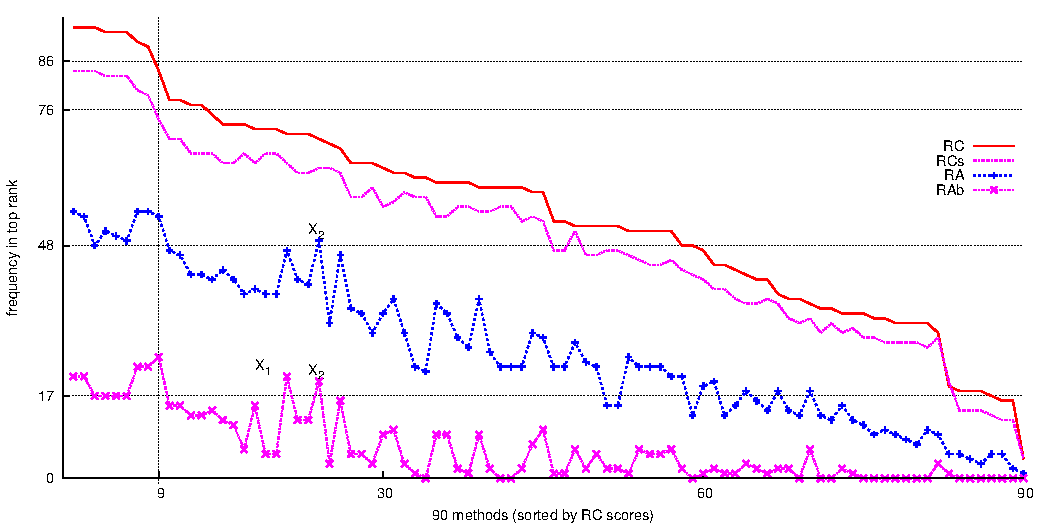
\includegraphics[width=6in]{row-numers.pdf}
\end{center}
\caption{How often 90 effort estimation methods were ranked \#1.
Recall that RC
uses a recursive Cohen test.
 RCs is the same as RC but with an addition
bootstrap test.
 RA is a
recursive ANOVA
test.
 RAbl uses
 the test recommended by Mittas and Angelis; i.e.
 recursive ANOVA with a Blom transform to convert all numerics to a Gaussian
distribution.
}\label{fig:results}
\end{figure*}


These 90 methods were assessed in
 leave-one-out-experiments using the data sets of \fig{datasets}.
Method performance was assessed via a range of
 performance measures. Let each
prediction models generate prediction $p_i$ for  $t$ test instances $i$.
If $|p_i - a_i|$ is $AR_i$ 
(the  {\em absolute residual}  difference between  predictions and actuals)
then:
\bi
\item
$MAR$ is the {\em mean absolute residual} $(\sum_i |p_i - a_i|)/t$.
\item
$MRE_i$ and $MER_i$ are the ratios  $AR_i/a_i$ and  $AR_i/p_i$.
\item
$PRED(X)$ is the percent of results with $MRE_i \le X\%$.
\item
$MMRE =\sum_i MRE_i/t$
\item
$MMER = \sum_i MER_i/t$.
\item
$MdMRE$ is median $MRE_i$ value. 
\item
Balanced errors
\mbox{$MBRE_i = (|p_i - a_i |)/ min(p_i,a_i)$} and \newline
\mbox{$MIBRE_i = (|p_i - a_i |)/ max(p_i,a_i)$}
\ei 

RC, RCs, RA, and RAbl were run separately on each data set.
Tallies were kept of how often a method was ranked \#1.
If all methods get the same rank (as seen in the {\em blurring}
effect of \tion{blur}),
then we declared that no method was ranked first.

\fig{results} shows  the 90 methods, sorted by how often they were
ranked \#1 by RC. 
In that figure, the RC and RCs curves are very similar.
RCs was implemented because we  mistrusted the simplicity of
the Cohen test. It turns out that a bootstrapping test rarely reports
any issues with the Cohen test; i.e. as argued by Shepperd \& MacDonell~\cite{shepperd12},
the Cohen test is a useful method to rank effort estimators. 


In \fig{results},
RA and RAbl produce  fewer
top ranked methods than the other approaches.
To see why,
we have examined 
numerous results from these different procedures.
It was seen that RA and RAbl often ``blur'' the results.
``Blurring'' was discussed in \tion{blur} and arises when the performance
of methods are indistinguishable. Blurring occurs for  
RA and RAbl when they try to distinguish very small sets of
methods that are remarkably better.  Consider one hundred
methods sorted by their mean score. If the first two methods
have mean scores 100 times less than the remaining, then RC will
isolate these two and give them a different rank to the rest.  RA and
RAbl, on the other hand, miss these small sets and assign them the
same ranks as the remaining methods.  

That said, in terms of functional equivalence, the differences between
RC, RCs, RA and RAbl are very small since the differences between
what methods are ranked best is very small.
To see this, consider what methods would be selected as ``better''
from \fig{results}.
In signal processing, it is standard  to segment data based on 
the region of maximal change~\cite{oppen96}. To apply this here, we 
sort 90 methods along an x-axis
in descending order of their score.
We then walk left to right across that plot
to find a region of steepest, most rapid change, followed by a 
lessening of those changes.
That steepest region marked the region of maximal change in the score and we will
use anything to the left of that region.
Note that this  procedure is quite effective: when  used in our recent IEEE TSE
article~\cite{me11a}, it selected methods that, when combined into an ensemble, out-performed
the individual methods.

The {\em vertical dashed line} in \fig{results}  shows
nine methods selected by this signal processing heuristic
from the RC curve.
An interesting feature of this heuristic is that it selects a very
small number of models: just those in the range 
\mbox{$1 \le x \le 9$}.
%% Note that only nine  of the 90
%% methods are selected as being ``better''.
%% This
%% This result The small size of the selected select is a result
%% of the nature of the performance of effort estimators.


\begin{figure}
\small
\begin{center}
 \begin{tabular}{l|l|ll}
\multicolumn{2}{c}{~}                      & learner    & pre-processor \\\hline
Group1& Deprecated           & SWReg      & width3bin\\
&(found in worst and not best)& Nnet& width5bin\\
&                      & PCR        & norm\\
&                      & PLSR       & SFS\\
&                      &            & freq3bin\\\hline
Group2&Recommended           & CART (yes) &\\
&(found in best 
but not worst)        & CART (no)  &\\
&                      & ABE0-5NN   &\\\hline
Group3&Mixed results         & ABE0-1NN   & PCA\\ 
&(no clear pattern)    & LReg       & SWReg\\
&                      &            & freq5bin\\
&                      &            & log\\
&                      &            & none
                    \end{tabular}
\end{center}
\caption{Across all statistical ranking procedures,
nearly the same estimators appeared in the top nine (the {\em best}
subset) and the bottom half (the {\em worst} subset).
}\label{fig:best}
\end{figure}



The {\em horizontal dashed lines}  show
what methods might be missed if we just focus on $1\le x \le 9$.
These lines  show the minimum y-values
for each statistical procedure in the same region $1\le x \le 9$.
The methods  $X_1$
and $X_2$ fall to the {\em right}  of $x=9$ and {\em above} 
the horizontal dashed lines. 
That is, these  methods might also be candidates for ``best'' method,
but are missed by the region $0\le x \le 9$. 
It is not clear what to make
of the $X_1$ and $X_2$
methods since the RA and RAbl curves are not 100\% confidence results.
If ANOVA
is applied with 95\% confidence to the 90 methods in \fig{results}, and if
we assume equal-sized divisions of the methods, then our total confidence
in the RA and RAbl curves is $A=0.95^{log_290}=72\%$; i.e.  the actual
position of $X_1$ and $X_2$ is not certain.


\fig{best} shows what learners and pre-processors were recommended by all
four statistical ranking procedures. To make these recommendations,
we note that all the rankers agreed on the top and bottom ends of the sorts
of \fig{results}. If we define the top nine as {\em best} and the bottom half
as {\em worst}, then those groups are:
\be
\item The {\em depreciated} set: 
those that were absent in {\em best} but appeared in {\em worst}.
\item The {\em recommended} set:
those that were absent  in {\em worst} and appeared in {\em best}.
\item The {\em mixed} set (everything else).
\ee
\fig{best} might be used to define a default
estimation procedure (using \fig{best}'s Group2 learners while
avoiding \fig{best}'s  Group1 pre-processors).
That said, it is important to add that we 
strongly recommend that organizations
do not blindly accept \fig{best}. Rather, it is better practice to
explore a range of estimators on new data sets (or even ensembles
of estimators using the methods of~\cite{me11a}).


\begin{figure*}
\begin{center}
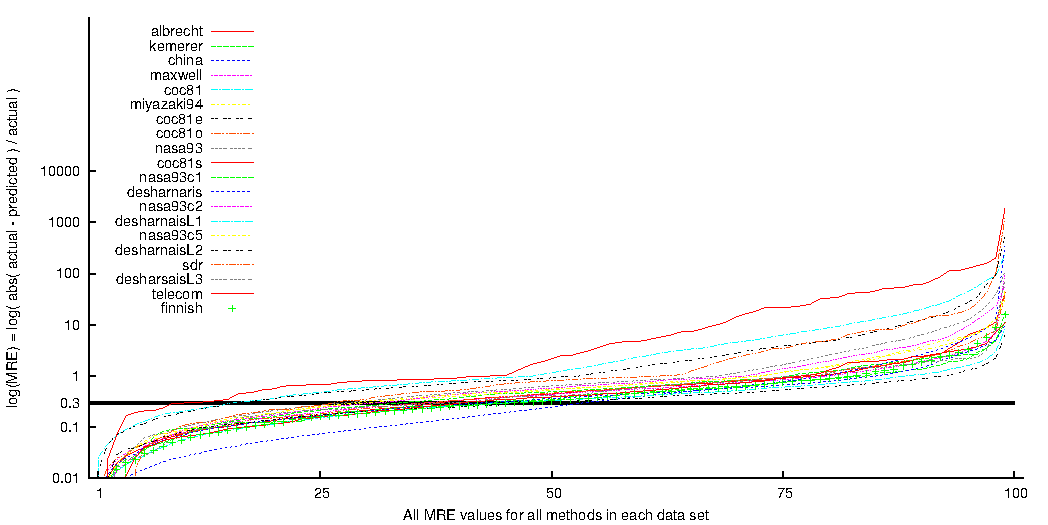
\includegraphics[width=6in]{mres.pdf}
\end{center}
\caption{Visualizing the space of MRE values.
Numerous methods are ``better'' and generate low errors
(MRE $<$ 10)\%
However, some methods are very bad and generate very large
errors (nearly a quarter have MREs over 100\%). }\label{fig:mres}
\end{figure*}


\section{Discussion}

%% XXX On thing we found in this study is that it
%% may be more  productive
%% to explore visualizations of software effort estimates than
%% relying on automatic algorithms to summarize that data.
%% For example, we can explain the above equivalence patterns via
%% a  {\em twin landscape}  effect that appears in our data. 
%% It turns out that the shape
%% of the performance scores generated by 
%% effort estimation methods two distinct zones:
%% \bi
%% \item A large ``lowlands'' of scores where effort estimation models achieve low error rates.
%% \item A smaller ``highlands'' of very large errors  where effort estimation models perform very
%% badly.
%% \ei
%% The rest of this pap 

The most startling feature of \fig{results} is that four different
statistical procedures offer similar rankings to 90 effort estimation
methods.  As mentioned above, if a method is top-ranked by one procedure,
it tends to have the same rank from the other procedures. Similarly,
at the other end of the spectrum, if a method is poorly-ranked by
one then it tends to be poorly ranked by all.  That is, 
while these methods differ in their fine-grained
conclusions, in the bigger scheme of things they are functionally
equivalent. 

How to explain this strange agreement between different
statistical procedures? One hypothesis is that the underlying data has
a very simple structure- so much so that different statistical methods
will always come to the same conclusion.
To test that, we graphed in \fig{mres} the MRE error measures generated by
our 90 methods on the 20 data sets used in this study.
In a result supporting the hypothesis of the previous paragraph,
we found a {\em twin landscape} effect:
\bi
\item
A few  left-hand-side {\em lowlands} results;
\item
Many  right-hand-side {\em highlands} results with very large errors.
\ei
This  highland region is even more  prominent than might be suggested
by \fig{mres}. Note that the y-axis of that figure uses a logarithmic scale--
so the right-hand-side highlands are very high indeed (many over 100\% error
and some with 1,000\% error or higher).

This twin landscape of performance scores explain the {\em
  conclusion instability} effect reported in a recent special issue of
the Empirical Software Engineering Journal~\cite{ci12}. 
In that special issue,
Menzies and Shepperd collected software engineering research papers
around the theme of ``what works there does not work here''.
The editorial of that issue proposed a long list of reasons
why such instability might exist. 
For the field of effort estimation, the results of this paper
offer a simpler, more direct explanation: \bi
\item Consider two research teams exploring effort estimation results
that  contain numerous large outliers (i.e.
performance scores from the ``highlands'').  
\item
For such data,
minor changes in how that data is processed
(e.g. in some cross-validation procedure) could mean that the two teams sample different groups
of the outliers.
\item Consequently, conclusions reached my one team may not be found by another.
\ei
Twin landscapes also explain  certain 
aberrant results in effort estimation.
Recently~\cite{koc13a}, we compared effort estimation
results from two kinds of validation experiments:   leave-one-out and cross-validation.
These experiments use test sets of different sizes:
\bi
\item Cross-validation tests
methods use a fraction of the data.
Cross-validation is problematic in that it
can introduce a confounding effect into effort estimation results
(when two research teams use different random number generators to build their cross-validation
test sets).
\item
Leave-one-out uses test sets of size $S=1$.
In theory, leave-one-out studies suffer from higher variance than
cross-validation (variance can grow very large as a test set shrinks since $\sigma \propto \frac{1}{S}$).
\ei
Strangely, 
we found no significant difference between the  variance
seen in these two kinds of experiments.
This is an important result since it means researchers are free to use leave-one-out, thus
avoiding the confounding effect of cross-validation. This result runs counter
to established statistical results~\cite{Mendes2007}
raising the question ``what is so unusual
about effort estimation results?''. 
 Note that,  in twin landscape data, 
we would expect very large variances in {\em both}
leave-one-out and cross-validation due to the
large frequency of the large errors. 




%% Finally, we discuss a seperate issue.
%% Suppose the goal is to find the single ``best'' model- how
%% should that task be performed?
%% A repeated result 
%% is that there is no ``best'' effort model that
%% scores best on all  criteria, on all data
%% sets~\cite{myrtveit05,me11a}.  Hence it is
%% a waste of time to seek
%% the single ``best'' model.  Rather,
%% when working with single estimators, the goal should  be
%% to avoid demonstrably
%% inadequate models.  Recall from \fig{results} and \fig{mres}  that
%% there exists a small number of left-hand-side candidate models that
%% are much better than the rest.  When using single models, any of these
%% better candidates will suffice. Note that the
%%  RC procedure recommended by this paper
%% can  find that small set of 
%% better candidates.


\section{Conclusions}

This paper has been about the functional equivalence of a set
of ranking procedures for software effort estimation: two
ranking procedures are functionally equivalent if they give
the same answers.  It has been shown that for effort
estimation, seemingly sophisticated
ranking procedures (including a bootstrapping approach and a Blom
transform) are functionally equivalent to a very simple
Cohen procedure.

This paper has {\em not} shown that {\em all} statistical methods
for all MSR tasks are needlessly elaborated. However, it
does raise the possibility that this might be the case. 
Hence, it is hoped
that other researchers will accept the challenge of this paper to
explore that issue for other MSR tasks and other ranking procedures.



As to the specific applications of this paper, we can use 
functional equivalence (defined in the introduction)
in two ways. Firstly, as shown in the {\em Discussion}
section, we can explain certain previously
inexplicable results (conclusion instability and the
similar performance of leave-one-out and cross-validation).

Secondly, we can use functional equivalence to  quick
prune 
research dead-ends before researchers waste  scarce
resources on tasks with little practical impact.
For example,
recent results propose the use of a Blom transform for
handling non-Gaussian distributions~\cite{mittas12a}.  
But, as discussed above,  Beasley and Erickson~\cite{beasley09} are concerned
that the Blom transform  has yet to be adequately certified.
Given
these two papers, a researcher might be tempted to explore these two
opposing viewpoints, perhaps using a simulation-style analysis 
(as done in Beasley and Erickson~\cite{beasley09} or Shepperd and Kadoda~\cite{shepperd01}).
 However, the results of this paper is that functionally equivalent
rankings are generated with and without the Blom transform- a
result suggesting that there is little practical benefit in debating
this particular ranking scheme for effort estimation.

As to future work, the external validity of this paper
needs to be explored
by repeating this study
for other ranking methods and other
MSR-style  tasks (defect detection, text mining,
etc). This paper suggests (but does not prove)
that it may be possible to significantly reduce the
complexity of at least some of the tools used for mining
software repositories.




%% We also endorse the RC procedure since  other procedures 
%% make recommendations to some limited level of confidence
%% \mbox{$\alpha < 100$\%}. 
%% On the other hand,  RC  {\em has no confidence limits}
%% (it just compares two means against
%% the standard deviation). 
%% Initially, we were concerned that RC was too simplistic but the RCs results
%% of \fig{results} show that, when we double-check the RC conclusions with bootstrap sampling,
%% then the overall results barely change. 

%% As to future work, there are some aspects of RC that deserve further
%% attention. For example,
%% RC is dependent on the Cohen threshold which, in this work, we have set to $0.3*\sigma$
%% (the standard deviation of the whole population). 
%% We know from \fig{results} that this setting produces very similar results to more sophisticated
%% approaches so, at least for this paper, we were not motivated to explore this matter.
%% However, in future work, it would be useful to check the critically of that  threshold.

%% But more importantly, RC simplifies effort estimation. Can it do the same for other
%% areas of software engineering?   This seems like an important direction for future work.


% argument is your BibTeX string definitions and bibliography database(s)
%
% <OR> manually copy in the resultant .bbl file
% set second argument of \begin to the number of references
% (used to reserve space for the reference number labels box)
%\bibliography{new}


{\small

\bibliographystyle{plain}
\bibliography{new}}

\section*{APPENDIX: Python code for RC}
This section shows a full implementation of
RC, using Python 2.7.1 (to download, see
http://goo.gl/AX0aJ).
This code runs on data of the form shown in \fig{rcdemo}. If successfully downloaded and installed,
the following interaction should be seen:

\begin{minipage}{0.7\linewidth}
\scriptsize
\begin{verbatim}

$ python rcdemo.py 
Demo1: finds three ranks
"x5" : [0.1, 0.2, 0.3, 0.4] mean = 0.25 rank = #1
"x3" : [0.15, 0.25, 0.35, 0.4] mean = 0.2875 rank = #1
"x1" : [0.34, 0.49, 0.51, 0.6] mean = 0.485 rank = #2
"x2" : [0.6, 0.7, 0.8, 0.9] mean = 0.75 rank = #3
"x4" : [0.6, 0.7, 0.8, 0.9] mean = 0.75 rank = #3
\end{verbatim}
\end{minipage}

\begin{minipage}{0.7\linewidth}
\scriptsize
\begin{verbatim}
Demo2: finds one rank (a.k.a. blurring)
"y1" : [99, 99.5, 100, 101, 101] mean = 100.1 rank = #1
"y2" : [99, 100, 100, 101, 101] mean = 100.2 rank = #1
"y3" : [99, 99.5, 100, 101, 101] mean = 100.1 rank = #1
"y4" : [99, 100, 100, 101, 101] mean = 100.2 rank = #1
\end{verbatim}
\end{minipage}




\noindent
\fig{bag} shows a  class that
 summarizes numbers; e.g. 
\[\mbox{\tt bag1 = Bag("method1",[10,20,30,40])}\]
generates
{\tt bag1} that knows the mean and standard deviation of \{10,20,30,40\}.
These objects
can   sort themselves based on their mean value (see {\tt \_\_lt\_\_})
and can  add and subtract from each other (see
{\tt \_\_add\_\_} and {\tt \_\_sub\_\_}).



Our {\tt rc} procedure, shown top of \fig{rfun}, 
is just
 a small variant
of the  {\tt r} procedure.
The main call of {\tt r} 
sorts the {\tt Bag}s then calls  
{\tt recurse} to explore any subset of the {\tt Bag}s 
that are better than the rest.
At each step of {\tt recurse}, the  
{\tt split} function  checks all divisions of a sorted list
of {\tt Bag}s.

Recursive exploration  should try
to avoid needless repeated analysis at every sub-level. Hence,
 when {\tt split} returns a cut-point,
it also returns a summary of the data to the left and right
of that split. These summaries are passed to recursive call-
which means that {\tt split} never has to re-compute a global summary.



This code separates the  {\tt r} procedures the  control options 
defined in the class {\tt R} (see \fig{rclass}).
These control options evaluate a division of  sorted list of bags {\tt oneTwo}
into two sublists {\em one} and {\em two}. 
For this evaluation, {\tt R} uses 
the sum of the squares of the differences
before and after the division
(see the {\tt now} function).  



We define these control options as in a separate (to
enable 
experimentation on different ways to rank effort estimators). 
The {\tt RC} class of \fig{rclass} shows what is unique
about the recursive Cohen test.
As shown in {\tt \_\_init\_\_}, 
when an instance of the {\tt RC} class is initialized, it computes and caches
the standard deviation of all scores (which is used
in the Cohen test, at end of {\tt different}). 
\codeb{rcdemo.py : demo code.}{rcdemo}
\codeb{The {\tt Bag} class}{bag}

\codeb{rfun.py : the {\tt r} and {\tt rc} procedures.}{rfun}
\codeb{rclass.py : control options for {\tt r} and {\tt rc}. }{rclass}


%\balancecolumns % GM June 2007
% That's all folks!
\end{document}
